\documentclass[11pt]{article}

\usepackage[margin=1in]{geometry}
\usepackage[T1]{fontenc}
\usepackage[utf8]{inputenc}
\usepackage{lmodern}
\usepackage{microtype}
\usepackage{setspace}
\usepackage{amsmath,amssymb,amsthm,mathtools}
\usepackage{booktabs,longtable,array}
\usepackage{enumitem}
\usepackage{graphicx}
\usepackage[authoryear,round]{natbib}
\usepackage{xcolor}
\usepackage[colorlinks=true,allcolors=blue!55!black]{hyperref}
\usepackage{url}

\onehalfspacing
\setlist[itemize]{leftmargin=1.6em,itemsep=0.25em,topsep=0.35em}
\setlist[enumerate]{leftmargin=1.8em,itemsep=0.25em,topsep=0.35em}
\renewcommand{\arraystretch}{1.15}

\newtheorem{assumption}{Assumption}
\newtheorem{definition}{Definition}
\newtheorem{lemma}{Lemma}
\newtheorem{proposition}{Proposition}
\newtheorem{corollary}{Corollary}
\newtheorem{conjecture}{Conjecture}
\theoremstyle{remark}
\newtheorem{remark}{Remark}
\newtheorem{observation}{Numerical observation}

\newcommand{\A}{\mathsf{A}}
\newcommand{\D}{\mathsf{D}}
\newcommand{\E}{\mathbb{E}}
\newcommand{\dd}{\,\mathrm{d}}

\title{Working Research Note II:\\Inequality and Political Regimes as a Joint Dynamic State\\[0.3em]
\large A re-evaluation of the modeling strategy, built on B\'enabou's log-normal workhorse}
\author{Draft for discussion}
\date{5 October 2026}

\begin{document}
\maketitle

\begin{abstract}
The previous note proposed a recursive incomplete-markets (Aiyagari/Krusell--Smith) economy and treated \citet{PerssonTabellini2009} as having pre-empted joint dynamic models of democracy and development.  Both choices were wrong for this project.  The aim is the two-way feedback between political regime and income distribution, not the aggregation of rich individual heterogeneity, and Persson and Tabellini's ``democratic capital'' is a reduced-form stock.  This note re-evaluates the model space using the log-normal, constant-elasticity machinery of \citet{Benabou1996,Benabou2000,Benabou2002}.  In that machinery the whole income distribution is summarized exactly by one number, and policy moves the future distribution through a single channel: intergenerational persistence.

The organizing result is a closed-form decomposition.  The elite's surplus from democracy equals the median's surplus minus a \emph{dynastic distributive stake} that is linear in inequality.  From this decomposition and the direction in which each regime moves inequality follow four results.  (i) A \emph{loop-sign} classification says when a regime reinforces or undermines itself.  (ii) Exact conditions for democratic consolidation are derived, including a closed-form time to consolidation and a declining breakdown hazard; this microfounds ``democratic capital'' as the inequality state, whose depreciation rate is the squared intergenerational persistence.  (iii) A closed-form phase diagram yields history dependence, democratic convergence, autocratic convergence and recurrent switching.  (iv) The previous note's mechanism (elites accept democracy for productive reasons) lives on a branch where both regimes undermine themselves.  On that branch, a forward-looking equilibrium destroys the regime cycles that myopic calculations predict.  All closed forms are checked against a Monte Carlo population and a numerical Markov-perfect solution; numerical findings are labeled as such.
\end{abstract}

\tableofcontents
\newpage

%=====================================================================
\section{Bottom line}
%=====================================================================

\paragraph{What changes relative to the previous note.}
\begin{enumerate}
\item \textbf{Drop Aiyagari.}  Agreed.  An Aiyagari economy earns its keep when the object of interest is how individual heterogeneity (precautionary saving, borrowing limits, idiosyncratic risk) aggregates into prices and quantities.  Here the object is a \emph{feedback loop}: the regime shapes the distribution, and the distribution shapes the incentives of whoever can change the regime.  For that we need a distribution that is (R1) endogenous to the regime's policy, (R2) payoff-relevant for the groups that control regime change, and (R3) summarized \emph{exactly} by a few statistics, so that regime decisions can be characterized rather than approximated.  B\'enabou's framework satisfies all three.
\item \textbf{Drop democratic capital as a primitive, and stop treating Persson--Tabellini as pre-emptive.}  The persistence result in \citet{PerssonTabellini2009} rests on an accumulated stock whose law of motion and effect on exit hazards are assumed.  That was too much weight to give it as a reason to set aside equilibrium joint models.  In the B\'enabou economy below, an object with exactly that accumulation structure arises endogenously.  Cross-sectional inequality evolves as a regime-switching AR(1), and its distance from the democratic steady state is the state that governs the coup hazard.  So ``democratic capital'' can be \emph{derived}, with testable restrictions (Section~\ref{sec:democap}).
\item \textbf{Keep the discipline of the old note.}  The imitation lemma and the ``democratize-then-harvest'' logic survive and become sharper in this setting.  Section~\ref{sec:productive} shows they are exactly what breaks the productive-democratization mechanism in a forward-looking equilibrium.
\end{enumerate}

\paragraph{Recommended core model.}  A B\'enabou economy has dynasties, log-normal human capital, credit-constrained investment in children out of post-tax income, and constant-elasticity redistribution.  Two regimes differ in who sets policy, and transitions are Acemoglu--Robinson style: the elite can stage coups against democracy, and the masses can threaten revolution against autocracy.  The state is $(\Delta^2,r)$: the cross-sectional variance of log income and the inherited regime.  Everything a regime decision needs is in closed form.

\paragraph{Main results (status in brackets).}
\begin{enumerate}
\item \emph{Surplus decomposition} [exact].  $S_E(\Delta)=S_M(\Delta^2)-(B_\A-B_\D)\,z\Delta$.  The elite's surplus from democracy equals the median's surplus (redistribution of current inequality, insurance against future luck, efficiency, minus deadweight) minus a dynastic distributive stake.  The stake is the elite's rank $z$ times inequality times the difference in how long each regime lets an advantage persist.  $S_E$ is U-shaped: a \emph{distributive branch} where it falls with inequality and a \emph{productive branch} where it rises.
\item \emph{Loop-sign principle} [exact, elementary].  Democracy compresses inequality and autocracy widens it.  Hence democracy reinforces itself on the distributive branch.  Autocracy undermines itself under revolution threats and reinforces itself under elite control.  On the productive branch, both regimes undermine themselves.
\item \emph{Consolidation and derived democratic capital} [exact local conditions; hazard formula verified numerically].  Democracy is locally stable iff $S_E(\Delta^*_\D)>-\psi$.  A democracy born inside the coup zone consolidates after $T(\Delta_0)$ periods, given in closed form, so the breakdown hazard falls with democratic age.
\item \emph{Phase diagram} [three of four regions exact; fourth numerical].  In (luck, coup-cost) space, closed-form boundaries separate four regions: history dependence (both regimes stable), democratic convergence, autocratic convergence, and recurrent switching.  The Markov solution agrees at 52 of 63 test points.  Wherever they differ, the equilibrium is \emph{more} stable than the closed form predicts, because of cross-regime anticipation: a fragile democracy stabilizes autocracy, and a fragile autocracy stabilizes democracy.
\item \emph{Two surprises from computation} [numerical].  (a) On the productive branch, myopic comparisons predict regime cycles.  The forward-looking equilibrium has none when reversals are cheap, because democracy then has no commitment value.  When reversals are only occasional, best-response iteration never settles on a pure-strategy Markov equilibrium.  (b) A stronger education channel ($\beta$) makes consolidation \emph{harder} in our calibration.  It speeds up inequality compression, but it raises the elite's dynastic stake by more, because democracy erodes the persistence of the elite's descendants' advantage.
\end{enumerate}

\paragraph{What this note cannot do.}  I could not read the Obsidian map (it is a local Windows path), so I infer the ``two one-sided literatures'' to be: (a) distribution/income $\to$ regime (modernization, redistributive-threat and elite-competition theories, and their empirical tests); and (b) regime $\to$ income/distribution (democracy and growth, democracy and redistribution/inequality).  If the map draws the line differently, Section~\ref{sec:empirics} is the part to revisit.  I also could not access the full text of \citet{Benabou2000} from this environment.  Statements about what it does and does not endogenize rest on memory and on secondary descriptions, and should be checked.

%=====================================================================
\section{What a joint model must do}\label{sec:requirements}
%=====================================================================

The two one-sided literatures each hold the other side fixed.  Theories of democratization take inequality as a parameter (\citealp{AcemogluRobinson2000,AcemogluRobinson2001,AcemogluRobinson2006}; \citealp{Boix2003}; \citealp{AnsellSamuels2014}).  Studies of democracy's effects take regime change as a treatment \citep{AcemogluEtAl2015Handbook,AcemogluEtAl2019JPE}.  Three equilibrium effects then go missing.
\begin{enumerate}
\item \textbf{State dependence.}  The effect of democratization on inequality depends on where inequality starts relative to the democratic steady state.  The effect of inequality on the regime depends on which group controls the transition.  Both ``effects'' are equilibrium functions of the joint state, not structural constants.
\item \textbf{Selection by the induced distribution.}  The regimes we observe surviving are those whose own policies produced a distribution that sustains them.  Before--after comparisons around transitions mix the treatment effect with this selection.
\item \textbf{Anticipation across regimes.}  The value of overturning a regime depends on how long the new regime will survive, which depends on the distribution it will create.  A model with one side exogenous cannot generate this.
\end{enumerate}
A model that delivers these needs (R1)--(R3) from the bottom line and nothing more.  Aiyagari delivers (R1)--(R2) at the cost of (R3).  Democratic-capital models deliver persistence by assuming the stock.  B\'enabou's framework delivers all three.

%=====================================================================
\section{The workhorse: a B\'enabou economy}\label{sec:workhorse}
%=====================================================================

\subsection{Environment}

Time is discrete; a period is a generation.  A unit mass of dynasties $i$ has log human capital $\ln h_{it}=m_t+x_{it}$, where $m_t$ is the cross-sectional mean of logs and $x_{it}$ the dynasty's position, with $x_{it}\sim N(0,\Delta_t^2)$ across dynasties.  Pre-tax income is $y_{it}=h_{it}$.

\paragraph{Redistribution.}  A policy $\tau$ (``progressivity'') maps pre-tax into post-tax income by
\begin{equation}
\hat y_{it}=y_{it}^{1-\tau}\,\tilde y_t^{\,\tau},
\qquad
\int \hat y_{it}\,\dd i=e^{d(\tau)}\int y_{it}\,\dd i ,
\label{eq:scheme}
\end{equation}
where $\tilde y_t$ balances the budget and $d(\tau)\le 0$, $d(0)=0$, is a deadweight loss.  It stands in for the labor-supply distortion in \citet{Benabou2000}; we use $d(\tau)=-\theta\tau^2/2$.  This is the tax function later popularized by \citet{HeathcoteStoreslettenViolante2017}, whose U.S.\ estimate of $\tau$ is about $0.18$.  $\tau<0$ is regressive.

\paragraph{Investment and credit constraints.}  Parents cannot borrow against children's earnings.  They invest a share $\sigma$ of post-tax income in the child, and
\begin{equation}
\ln h_{i,t+1}=\kappa+\alpha\ln h_{it}+\beta\ln(\sigma\hat y_{it})+\varepsilon_{i,t+1},
\qquad \varepsilon\sim N(0,s^2)\ \text{i.i.d.},
\label{eq:hk}
\end{equation}
with $\alpha,\beta>0$ and $a\equiv\alpha+\beta<1$.  Here $\alpha$ is direct transmission (genes, culture, networks), $\beta<1$ the concave return to parental investment, and $s^2$ the variance of ``luck.''

\paragraph{Preferences.}  Dynasties maximize $\E\sum_{t\ge0}\delta^t\ln c_{it}$ with $c_{it}=(1-\sigma)\hat y_{it}$.  A constant $\sigma$ is a tractability assumption.  With log utility and the technology~\eqref{eq:hk}, the optimal share is common across dynasties and depends only on the aggregate policy path.  It would therefore add regime-specific constants but would not affect the distribution of positions.

\paragraph{Notation.}  Let
\[
g(\tau)=\tfrac{\tau(2-\tau)}{2},\quad
\rho(\tau)=\alpha+\beta(1-\tau),\quad
\omega=\frac{1-\delta\alpha}{1-\delta a},\quad
\Pi(\tau)=\frac{\omega\,g(\tau)}{1-\delta\rho(\tau)^2},\quad
B(\tau)=\frac{1-\tau}{1-\delta\rho(\tau)} .
\]

\subsection{Exact aggregation}

\begin{lemma}[Exact aggregation]\label{lem:agg}
If $x_{t}\sim N(0,\Delta_t^2)$ and policy is $\tau_t$, then
\begin{align}
\ln\hat y_{it}&=d(\tau_t)+m_t+(1-\tau_t)\,x_{it}+g(\tau_t)\,\Delta_t^2, \label{eq:posttax}\\
x_{i,t+1}&=\rho(\tau_t)\,x_{it}+\varepsilon_{i,t+1}, \label{eq:position}\\
\Delta_{t+1}^2&=\rho(\tau_t)^2\,\Delta_t^2+s^2, \label{eq:variance}\\
m_{t+1}&=\text{const}+a\,m_t+\beta\big[d(\tau_t)+g(\tau_t)\Delta_t^2\big]. \label{eq:mean}
\end{align}
\end{lemma}

\begin{proof}
With $\ln h\sim N(m,\Delta^2)$, the budget in \eqref{eq:scheme} reads $\tau\ln\tilde y+(1-\tau)m+(1-\tau)^2\Delta^2/2=d+m+\Delta^2/2$.  Hence $\ln\tilde y=m+d/\tau+(2-\tau)\Delta^2/2$, and substituting into $\ln\hat y=(1-\tau)\ln h+\tau\ln\tilde y$ gives \eqref{eq:posttax}.  Inserting \eqref{eq:posttax} into \eqref{eq:hk} and separating the mean from deviations gives \eqref{eq:position}--\eqref{eq:mean}.  Normality is preserved, so the argument applies every period.
\end{proof}

\paragraph{What each term means.}  Policy reaches the future distribution only through the persistence $\rho(\tau)$, which is the intergenerational elasticity of income.  Redistribution lowers it because, under credit constraints, it reallocates investment resources toward poor families.  The term $\beta g(\tau)\Delta^2$ in \eqref{eq:mean} is the \emph{efficiency gain} from redistribution.  Because returns to parental investment are concave ($\beta<1$), equalizing investment raises mean log human capital, and the gain is proportional to inequality.  One can check that aggregate human capital in levels rises with small $\tau>0$ iff $a<1$.

\begin{lemma}[Closed-form dynastic values]\label{lem:values}
Along any deterministic policy sequence $\{\tau_{t+k}\}_{k\ge0}$, the value of a dynasty at position $x$ is
\begin{equation}
V=\frac{m_t}{1-\delta a}+\sum_{k\ge0}\delta^k\,\omega\big[d(\tau_{t+k})+g(\tau_{t+k})\Delta^2_{t+k}\big]
+\Big[\sum_{k\ge0}\delta^k(1-\tau_{t+k})\prod_{j<k}\rho(\tau_{t+j})\Big]x+\text{const}.
\label{eq:Vgeneral}
\end{equation}
Under a permanent regime $r$ with policy $\tau_r$,
\begin{equation}
V_r(x,\Delta^2)=\frac{m_t}{1-\delta a}+C_r+\Pi_r\,\Delta^2+B_r\,x+\text{const},\qquad
C_r=\frac{\omega\,d(\tau_r)}{1-\delta}+\Pi_r\frac{\delta s^2}{1-\delta}.
\label{eq:Vperm}
\end{equation}
\end{lemma}

\begin{proof}
Sum the flow utility $\ln\hat y$ from \eqref{eq:posttax}.  Define $M=\sum_k\delta^km_{t+k}$; then \eqref{eq:mean} gives $M=[m_t+\delta\sum_k\delta^k\beta(d+g\Delta^2)_{t+k}]/(1-\delta a)$, and $1+\delta\beta/(1-\delta a)=\omega$.  Positions follow \eqref{eq:position}, so $\E_t x_{t+k}=\prod_{j<k}\rho_{t+j}\,x_t$.  For \eqref{eq:Vperm} use $\sum_k\delta^k\Delta^2_{t+k}=\Delta^2/(1-\delta\rho^2)+\delta s^2/[(1-\delta)(1-\delta\rho^2)]$.
\end{proof}

A Monte Carlo population of 400{,}000 dynasties, run through a regime switch with the exact budget-balancing transfer, reproduces \eqref{eq:Vgeneral}.  The slope in $x$ is $1.033$ against $1.035$ in closed form; the intercept is $0.316$ against $0.315$.

\paragraph{The three channels of policy value.}  In \eqref{eq:Vperm}, $\Pi_r\Delta^2$ is the value of redistributing \emph{current} inequality, inclusive of the efficiency gain (the factor $\omega>1$).  $\Pi_r\,\delta s^2/(1-\delta)$ is \emph{insurance} against future luck.  $B_r x$ is the \emph{dynastic stake}: how much a position is worth, which depends on both the retention rate $1-\tau$ and how long the regime lets the advantage persist ($\rho_r$).  Only the last term differs across dynasties.

\begin{proposition}[Common efficiency]\label{prop:common}
For any two policy sequences, the difference in value is $V-V'=(\text{term common to all dynasties})+(B-B')\,x$.  Hence (a) the efficiency and insurance effects of policy are valued identically by every dynasty; (b) preferences over policy sequences are ordered by the single index $x$ (single crossing); and (c) dynasties disagree about policy \emph{only} through their distributive stakes.
\end{proposition}
\begin{proof}
Immediate from \eqref{eq:Vgeneral}: $m_t$, the $\omega[\cdot]$ terms and constants do not depend on $x$.
\end{proof}

Proposition~\ref{prop:common} is important for the productive-democratization idea (Section~\ref{sec:productive}).  In this class of economies, the productive gains from redistribution can never be the reason one group wants \emph{another} group to hold power: everyone values them equally.  Delegation can be valuable only if the delegating group cannot control future policy itself, or if a de facto threat forces its hand.

%=====================================================================
\section{The organizing principle: surpluses and loop signs}\label{sec:loops}
%=====================================================================

Fix two regimes.  Under autocracy $\A$ the policy is $\tau_\A$, chosen by an elite; under democracy $\D$ it is $\tau_\D>\tau_\A$, chosen by the median.  In the core model these are a fixed policy menu: the regime is a bundle of de jure rules that includes its fiscal constitution.  Section~\ref{sec:menu} discusses endogenous policies.  The elite is the group at rank $z$ in the current distribution, i.e.\ at position $x_E=z\Delta$ (e.g.\ $z=2.33$ for the top 1\%).  The median dynasty is at $x=0$.  Let $\Delta^{*2}_r=s^2/(1-\rho_r^2)$ be regime $r$'s steady-state inequality; $\rho_\D<\rho_\A$ implies $\Delta^*_\D<\Delta^*_\A$.

\begin{proposition}[Surplus geometry]\label{prop:surplus}
Comparing permanent regimes, the median's and the elite's surplus from democracy are
\begin{align}
S_M(\Delta^2)&=\underbrace{\frac{\omega\,[d(\tau_\D)-d(\tau_\A)]}{1-\delta}}_{\text{deadweight}\ (<0)}
+(\Pi_\D-\Pi_\A)\Big[\underbrace{\Delta^2}_{\text{current inequality}}+\underbrace{\tfrac{\delta s^2}{1-\delta}}_{\text{insurance}}\Big],\label{eq:SM}\\
S_E(\Delta)&=S_M(\Delta^2)-\underbrace{(B_\A-B_\D)\,z\,\Delta}_{\text{dynastic stake}}.\label{eq:SE}
\end{align}
If $\Pi_\D>\Pi_\A$ (true whenever $\tau_\A\le 0<\tau_\D<1$), then $S_M$ is increasing in $\Delta^2$.  Since $B_\A>B_\D$, $S_E$ is a convex parabola in $\Delta$ with minimum at
\begin{equation}
\hat\Delta=\frac{(B_\A-B_\D)\,z}{2(\Pi_\D-\Pi_\A)}.
\label{eq:Dhat}
\end{equation}
It is decreasing on $[0,\hat\Delta)$ (the \emph{distributive branch}) and increasing beyond (the \emph{productive branch}).
\end{proposition}
\begin{proof}
Difference \eqref{eq:Vperm} across regimes at $x=0$ and at $x=z\Delta$.  $B(\tau)$ is decreasing in $\tau$ because the numerator falls and the denominator rises.
\end{proof}

\begin{figure}[t]
\centering
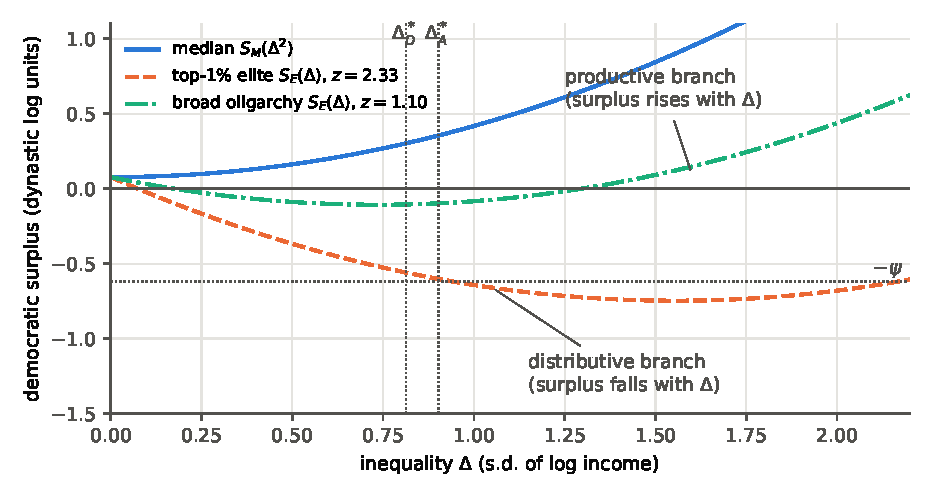
\includegraphics[width=0.85\textwidth]{figures/fig1_surplus.pdf}
\caption{Democratic surpluses in the baseline calibration (Table~\ref{tab:calib}).  The top-1\% elite ($z=2.33$, $\hat\Delta=1.56$) sits on the distributive branch over the empirically relevant range, around $\Delta^*_\D=0.81$ and $\Delta^*_\A=0.90$.  A broader oligarchy ($z=1.10$, $\hat\Delta=0.74$) reaches the productive branch.  The dotted horizontal line marks a coup cost $\psi=0.62$; the elite stages a coup where its surplus lies below $-\psi$.}
\label{fig:surplus}
\end{figure}

\paragraph{Interpretation.}  Democracy costs the elite through its stake, which grows linearly in $\Delta$.  It benefits the elite through the common terms that grow with $\Delta^2$.  These are the gain from compressing a log-normal distribution at a given mean (everyone's log income rises by $g(\tau)\Delta^2$ before netting out their position) and the efficiency gain (the factor $\omega$).  At very high inequality these common gains are large enough that even the rich gain.  The tension is closely related to the one behind the hump-shaped political support curve in \citet{Benabou2000}.  Here it is applied to the choice of \emph{who} sets policy rather than to the policy itself.  A narrow elite (large $z$) stays on the distributive branch; a broad oligarchy (small $z$) can reach the productive branch at realistic inequality.

\paragraph{Loop signs.}  Under each regime, inequality moves monotonically toward that regime's steady state, by \eqref{eq:variance}.

\begin{lemma}[Loop sign]\label{lem:loopsign}
Suppose regime $r$ can be overturned at random opportunity dates (probability $\pi_r>0$ per period), and that it is overturned at such a date iff $\Delta$ lies in an exit set $X_r$.  (i) If the interval between $\Delta_0$ and $\Delta^*_r$ is disjoint from $X_r$, the regime is never overturned.  (ii) If $\Delta^*_r$ is in the interior of $X_r$, it is overturned almost surely in finite time.
\end{lemma}
\begin{proof}
Under $r$, $\Delta_t$ moves monotonically from $\Delta_0$ to $\Delta^*_r$ by \eqref{eq:variance}.  In case (i) it never enters $X_r$.  In case (ii) it enters $X_r$ in finite time and stays there, and each period carries an exit probability of at least $\pi_r>0$.
\end{proof}

Combining Lemma~\ref{lem:loopsign} with Proposition~\ref{prop:surplus} gives the sign table below.  Democracy lowers $\Delta$ and autocracy raises it, and exit sets are upper or lower contour sets of a monotone surplus on each branch.

\begin{center}
\small
\begin{tabular}{llll}
\toprule
Regime & Who can overturn it & Distributive branch & Productive branch\\
\midrule
Democracy ($\Delta\downarrow$) & elite (coup) & self-reinforcing & self-undermining\\
Autocracy ($\Delta\uparrow$) & masses (revolution) & self-undermining & self-undermining\\
Autocracy ($\Delta\uparrow$) & elite (voluntary handover) & self-reinforcing (trap) & self-undermining\\
\bottomrule
\end{tabular}
\end{center}

The table is the ``Ah'' of the framework.  Whether a regime digs itself in depends on whether the inequality it generates strengthens or weakens the group that holds the key to its survival.  Democracy survives on the distributive branch because compressing inequality shrinks the elite's stake.  The previous note's mechanism lives on the productive branch, where it predicts instability rather than consolidation.  Democracy cures the inequality that made it worthwhile to the elite; this is the dynamic form of ``democratize, then harvest.''

%=====================================================================
\section{Re-evaluating the model space}\label{sec:menu}
%=====================================================================

All candidates below share the workhorse.  They differ in which transition technology closes the loop.  For each, I state the force, what it delivers, what kills it, and a verdict.

\subsection{M1. Coups and distributional consolidation (recommended core, democratic side)}
\emph{Force.}  The elite's coup incentive is its dynastic stake net of common gains.  Democracy erodes the stake by compressing inequality.  \emph{Delivers.}  Exact consolidation conditions, a closed-form time to consolidation, a declining hazard, and a derivation of democratic capital (Section~\ref{sec:core}).  \emph{Kills it.}  A steady-state democratic inequality inside the coup zone (high luck $s^2$, low coup cost).  \emph{Closest.}  \citet{AcemogluRobinson2001} (inequality raises coup incentives in a two-class model); \citet{PerssonTabellini2009} (persistence via an assumed stock).  \emph{Verdict.}  Core.

\subsection{M2. Revolution threats and inequality management (recommended core, autocratic side)}
\emph{Force.}  Autocracy raises inequality, which raises the masses' surplus $S_M$ until the revolution constraint binds.  This is the Acemoglu--Robinson channel, but with inequality as an endogenous state rather than a parameter.  \emph{Twist from the workhorse.}  A one-period concession has durable effects, because it lowers next period's inequality and raises mean human capital.  The computations clarify which durability matters.  The efficiency durability (the factor $\omega$) scales the value of a concession and of democracy alike, so it does not favor concessions.  What favors autocratic survival is the \emph{state} effect: concessions lower future $\Delta$ and thus future revolutionary pressure.  This gives a dynamic rationale for land reform and mass education under autocracy \citep{Grossman1994,Albertus2015,Paglayan2021} as \emph{inequality management}.  \emph{Kills it.}  With generation-length periods and $\delta=0.5$, a one-generation concession is very valuable.  With concessions allowed, democratization occurred in our runs only for $\mu\le0.1$.  Apart from the smallest cost ($\mu=0.05$, $q=0.1$), it occurred only when the resulting democracy would be safe from coups ($\psi=0.62$ rather than $0.45$).  The masses accept concessions rather than fight for a democracy that will not last.  With shorter periods (overlapping cohorts), the commitment problem bites harder.  \emph{Verdict.}  Core, but with concessions as an extension; near thresholds the numerical solution has convergence issues (Section~\ref{sec:numerics}).

\subsection{M3. Mobility and the elite's constitutional choice}
\emph{Force.}  A rank-defined elite's descendants regress toward the mean, so future autocratic rulers are \emph{other} dynasties.  The current elite may delegate future policy to the median to commit to a path closer to what its descendants will want \citep{JackLagunoff2006,Leventoglu2014,AcemogluEgorovSonin2018}.  \emph{Twist from the workhorse.}  Mobility is endogenous to policy, through $\rho(\tau)$.  \emph{Delivers.}  Approximate positional losses, $(\tau^*(x)-\tau^*(y))^2\propto(x-y)^2$, with a stationary $\Delta$ give a sharp condition.  The current elite prefers to delegate all future policy to the median iff $\sum_k\delta^k(1-2\rho^k)>0$, i.e.\ iff
\[
\delta\,(2-\rho)>1,
\]
independent of $z$ and $\Delta$.  With generation-length discounting ($\delta\approx0.5$) this never holds, so voluntary delegation needs patient dynasties relative to mobility.  Democracy lowers $\rho$, which loosens the condition: a mobility-based self-reinforcing loop.  \emph{Kills it.}  Low intergenerational discounting.  \emph{Verdict.}  Absorbed into the core as the $B_\A-B_\D$ term.  A stand-alone version needs endogenous Markov policies.

\subsection{M4. Productive democratization (the previous note's mechanism)}\label{sec:productive}
\emph{Force.}  Elites accept democracy because productive redistribution raises their returns.  \emph{What the workhorse says.}  By Proposition~\ref{prop:common}, productive gains are common to all dynasties, so on their own they never justify handing over power.  The mechanism therefore needs one of three things:
\begin{enumerate}[label=(\roman*)]
\item the elite's inability to control future policy (rank turnover, M3);
\item a hold-up of private decisions that respond to \emph{future} policy;
\item a de facto threat (M1/M2).
\end{enumerate}
Route (ii) is shut down in this class by construction.  With log utility and Cobb--Douglas investment, private investment shares do not respond to future retention rates in a way that differs across dynasties.  A hold-up version needs non-log utility, a discrete investment margin \citep[as in][]{GalorZeira1993}, or occupational entry.

\emph{What the forward-looking equilibrium says.}  With the elite controlling both directions (voluntary handover and coups), the computations give three findings.  Parameters: $\tau_\A=-0.25$, $\tau_\D=0.35$, $s^2=0.47$, $z=1.10$, so that $S_E$ is increasing on $[\Delta^*_\D,\Delta^*_\A]=[0.79,1.06]$ and crosses zero at $0.87$.
\begin{observation}\label{obs:productive}
(a) Permanent-value comparisons predict cycles: democratize when $\Delta$ rises above $0.87$, revert when it falls below.  (b) When reversals are frequent and nearly costless (coup opportunity every period; switching costs $0.005$--$0.02$), the forward-looking elite \emph{never} democratizes on $[0.79,1.06]$.  The handover threshold is about $1.18$--$1.19$, above $\Delta^*_\A$, so autocracy is absorbing.  A democracy the elite can undo at will is a one-period policy choice, not a commitment; the insurance and efficiency terms that drive $S_E$ accrue only while democracy lasts.  (c) With occasional reversal opportunities ($p=0.1$--$0.25$), best-response iteration on threshold strategies never settles.  This holds under damping from $0.5$ to $0.97$ and grids of $700$ and $1500$ points, which suggests that equilibrium requires mixed strategies (random regime switching).
\end{observation}
\emph{Verdict.}  Keep it as the productive branch of the core, where its job is to explain \emph{instability}.  To make it the centerpiece, add a primitive outside the log-linear class that creates a genuine hold-up.  That is a separate paper.

\subsection{M5. Endogenous policies within regimes: captured democracy}
\emph{Force.}  Let the democratic median choose $\tau$ each period subject to the elite's no-coup constraint, as in \citet{AcemogluRobinson2008}.  The constraint binds more tightly when inequality is high, because the stake is $\propto z\Delta$.  So the democratic policy is increasing in $\Delta$ where the constraint is slack and decreasing where it binds.  Combined with the decreasing steady-state locus $\Delta^{*2}(\tau)=s^2/(1-\rho(\tau)^2)$, this can produce multiple democratic steady states.  One is consolidated (low $\Delta$, high $\tau$, constraint slack); the other is captured (high $\Delta$, low $\tau$, constraint binding).
\begin{conjecture}
In the endogenous-policy version, democracy has two stable steady states for an open set of parameters.  Redistribution rises with democratic age along paths that consolidate.  A temporary leveling shock, such as a war or crisis destroying top wealth, can move a captured democracy into the consolidated basin.
\end{conjecture}
\emph{Status.}  Not computed.  \emph{Verdict.}  The natural second paper, or the second half of the first.  It is structurally close to \citet{Benabou2000}'s US/Europe multiplicity, so the contribution must be the de facto-constraint source of the hump, not the diagram.

\subsection{M6. Distribution-dependent de facto power}
\emph{Force.}  Repression or coup capacity scales with the elite's income share, which rises with $\Delta$.  Autocracy then reinforces itself even under revolution threats.  \emph{Risk.}  Easily becomes a reduced form; it is defensible only if repression is financed explicitly, e.g.\ by taxing elite income.  \emph{Verdict.}  Optional extension.

\subsection{Comparison}

\begin{longtable}{p{0.19\textwidth}p{0.22\textwidth}p{0.22\textwidth}p{0.25\textwidth}}
\toprule
Model & Loop (Section~\ref{sec:loops}) & Tractability & Main risk\\
\midrule
\endhead
M1 coups & D self-reinforcing & closed form & close to AR (2001) unless dynamics are the point\\
M2 revolutions & A self-undermining; concessions manage the state & closed form w/o concessions; numerical with & generation-length periods weaken the commitment problem\\
M3 mobility & D reinforces via $\rho$ & needs Markov policies & close to Jack--Lagunoff (2006)\\
M4 productive & both self-undermining & numerical; no pure-strategy equilibrium found & needs a hold-up primitive outside the class\\
M5 captured democracy & multiple D steady states & semi-closed form & relabeling of B\'enabou (2000) if not careful\\
M6 de facto power & A self-reinforcing & closed form & reduced-form repression technology\\
\bottomrule
\end{longtable}

%=====================================================================
\section{The core model}\label{sec:core}
%=====================================================================

\subsection{Environment, timing, equilibrium}

The economy is the workhorse with fixed menu $\tau_\A<\tau_\D$.  Each period:
\begin{enumerate}
\item The state $(\Delta_t^2,r_{t-1})$ is observed.
\item If $r_{t-1}=\D$, with probability $p$ the elite has a coup opportunity.  A coup installs $\A$ and costs the coup-staging elite $\psi$ (dynastic utility).  If $r_{t-1}=\A$, with probability $q$ the masses can revolt at cost $\mu$; revolution installs $\D$ and expropriates the elite.  The elite moves first and may democratize peacefully (or, in an extension, concede $\tau_\D$ for one period while keeping $\A$).
\item Regime $r_t$ sets $\tau_{r_t}$; incomes, consumption and investment follow Lemma~\ref{lem:agg}, and $\Delta_{t+1}^2=\rho(\tau_t)^2\Delta_t^2+s^2$.
\end{enumerate}
The masses are represented by the median dynasty and the elite by the rank-$z$ dynasty; costs are borne by the deciding group.

\begin{definition}[Markov equilibrium]
Decision rules depend on $(\Delta^2,r_{-1})$ and the opportunity draw.  Each decision maximizes the decider's dynastic value given the rules, and values are generated by the rules.  By Lemma~\ref{lem:values}, every equilibrium value is linear in the position, $W(\Delta^2,r)+B(\Delta^2,r)\,x$, so the state stays two-dimensional.
\end{definition}

\begin{table}[t]
\centering
\caption{Baseline calibration (a period is a generation)}\label{tab:calib}
\begin{tabular}{lll}
\toprule
Parameter & Value & Note\\
\midrule
$\alpha,\ \beta$ & $0.20,\ 0.45$ & $\rho_\A=0.65$, $\rho_\D=0.54$ (IGE range)\\
$\delta$ & $0.5$ & per generation\\
$\tau_\A,\ \tau_\D$ & $0,\ 0.25$ & HSV-type progressivity\\
$\theta$ & $1$ & deadweight $d(\tau)=-\theta\tau^2/2$\\
$s^2$ & $0.47$ & $\Delta^*_\A=0.90$, $\Delta^*_\D=0.81$\\
$z$ & $2.33$ & top 1\%\\
$p,\ q,\ \mu$ & $0.3,\ 0.3,\ 0.35$ & opportunities and revolution cost\\
Derived & $\omega=1.33$, $\Pi_\D=0.34$, $B_\A-B_\D=0.46$ & $\hat\Delta=1.56$\\
\bottomrule
\end{tabular}
\end{table}

\subsection{Consolidation and derived democratic capital}\label{sec:democap}

Let the coup zone be $Z=\{\Delta: S_E(\Delta)<-\psi\}$.  By Proposition~\ref{prop:surplus} it is an interval $(\Delta_C,\bar\Delta_C)$, possibly empty, with $\Delta_C<\hat\Delta<\bar\Delta_C$.

\begin{proposition}[Consolidation]\label{prop:consol}
Let autocracy be absorbing ($q=0$).
\begin{enumerate}[label=(\alph*)]
\item If the interval between $\Delta_0$ and $\Delta^*_\D$ does not meet $Z$, there is a Markov equilibrium in which a democracy born at $\Delta_0$ is never overthrown.  Democracy is locally stable at its steady state iff $S_E(\Delta^*_\D)>-\psi$.
\item Suppose the elite stages a coup at every opportunity inside $Z$; this holds in the computed equilibrium, whose threshold coincides with the closed-form $\Delta_C=0.943$.  Then a democracy born at $\Delta_0\in Z$ with $\Delta^*_\D<\Delta_C$ consolidates after
\begin{equation}
T(\Delta_0)=\left\lceil\frac{\ln\big[(\Delta_0^2-\Delta^{*2}_\D)/(\Delta_C^2-\Delta^{*2}_\D)\big]}{\ln(1/\rho_\D^2)}\right\rceil
\label{eq:T}
\end{equation}
periods.  It survives with probability $(1-p)^{T(\Delta_0)}$.  For a cohort of democracies with initial inequality drawn from $F$, the breakdown hazard at age $k$ is
\begin{equation}
h(k)=p\,\frac{\int \mathbf 1\{T(\Delta_0)>k\}\,(1-p)^k\,\dd F}{\int (1-p)^{\min\{T(\Delta_0),k\}}\,\dd F},
\label{eq:hazard}
\end{equation}
which is non-increasing in $k$ and zero for $k\ge\max T$.
\end{enumerate}
\end{proposition}
\begin{proof}
(a) If no future elite stages a coup, the elite's value of democracy is the permanent value, and on the path $S_E\ge-\psi$, so no elite wants to stage one; the conjectured rule is therefore consistent.  For the ``only if'' part: if democracy were absorbing near $\Delta^*_\D$ with $S_E(\Delta^*_\D)<-\psi$, the permanent-value comparison would make a coup strictly profitable, a contradiction.  (b) By \eqref{eq:variance}, $\Delta^2_k-\Delta^{*2}_\D=\rho_\D^{2k}(\Delta_0^2-\Delta^{*2}_\D)$; solve for the first $k$ with $\Delta_k\le\Delta_C$.  Surviving to age $k$ has probability $(1-p)^{\min(T,k)}$, and only democracies with $T>k$ face hazard $p$ at age $k$.
\end{proof}

\begin{corollary}[Democratic capital, derived]\label{cor:democap}
Write $\Delta^2_{t+1}-\Delta^{*2}_\D=\rho_\D^2(\Delta^2_t-\Delta^{*2}_\D)+\mathbf 1\{r_t=\A\}(\rho_\A^2-\rho_\D^2)\Delta_t^2$.  The ``inequality gap'' $\Delta^2_t-\Delta^{*2}_\D$ is a stock.  It is depleted under democracy at rate $1-\rho_\D^2$ and replenished under autocracy, and the breakdown hazard is $p\cdot\mathbf 1\{\Delta_t>\Delta_C\}$.  This is the structure \citet{PerssonTabellini2009} posit for democratic capital, with three testable restrictions:
\begin{enumerate}[label=(\roman*)]
\item the depreciation rate is one minus the squared intergenerational elasticity;
\item conditional on current inequality, past democratic experience does not predict breakdown, which separates this channel from values-based persistence;
\item the hazard falls faster where $\rho_\D$ is lower or $\Delta_C$ higher.
\end{enumerate}
\end{corollary}

In the calibration with $\psi=0.62$, $Z=(0.943,2.167)$.  For democracies born at $\Delta_0\sim U[0.85,1.6]$, the hazard is $0.26$ at age $0$ and $0.15$ at age $1$, then zero (Figure~\ref{fig:hazard}).  The Markov simulation and \eqref{eq:hazard} agree to the third decimal.  Ages are in generations because periods are; an overlapping-cohort version, in which a fraction of dynasties renews each period, rescales speeds without changing the structure.

\begin{figure}[t]
\centering
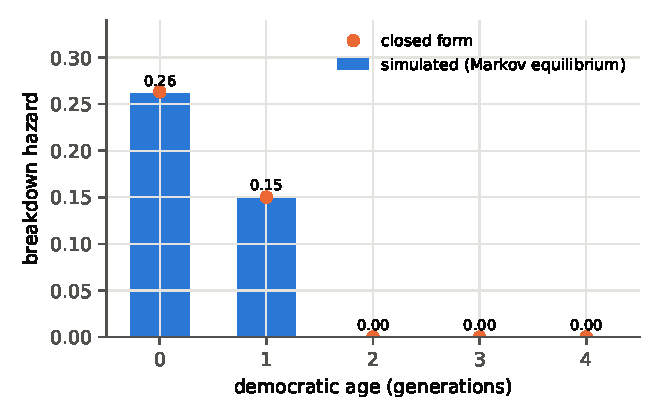
\includegraphics[width=0.55\textwidth]{figures/fig4_hazard.pdf}
\caption{Breakdown hazard by democratic age for democracies born at $\Delta_0\sim U[0.85,1.6]$ ($\psi=0.62$, $p=0.3$, autocracy absorbing).  Bars: simulated Markov equilibrium (40{,}000 democracies).  Dots: closed form \eqref{eq:hazard}.}
\label{fig:hazard}
\end{figure}

\paragraph{Comparative statics in the education channel.}  The natural intuition is that a stronger education channel helps democracy: redistribution then compresses inequality faster.  To check, raise $\beta$ while holding $\rho_\A=0.65$ fixed (so $\alpha=0.65-\beta$).  The result goes the other way:

\begin{center}
\begin{tabular}{cccccc}
\toprule
$\beta$ & $\rho_\D$ & $\Delta^*_\D$ & stake $B_\A-B_\D$ & $\psi_c=-S_E(\Delta^*_\D)$ & $T(1.5)$ at $\psi=0.62$\\
\midrule
0.25 & 0.588 & 0.847 & 0.420 & 0.529 & 1.08\\
0.35 & 0.562 & 0.829 & 0.438 & 0.545 & 1.35\\
0.45 & 0.538 & 0.813 & 0.456 & 0.560 & 1.56\\
0.55 & 0.512 & 0.798 & 0.473 & 0.574 & 1.75\\
\bottomrule
\end{tabular}
\end{center}
Here $T(1.5)$ is the uncapped ratio in \eqref{eq:T}.  The coup cost needed for consolidation rises, and so does the time to consolidate.  The force is the dynastic stake.  When policy shapes mobility more strongly, democracy erodes the persistence of the elite's descendants' advantage, which is precisely what the elite fights.  The coup zone expands faster than compression speeds up.  This is one calibration; the general statement is a boundary: a higher $\beta$ eases consolidation iff the compression effect on $\Delta^*_\D$ and on $\Pi_\D$ outweighs the rise in $B_\A-B_\D$.

\subsection{Autocratic stability}

\begin{proposition}[Autocratic stability]\label{prop:auto}
Let democracy be absorbing ($p=0$) and concessions unavailable.  Autocracy is locally stable at its steady state iff $S_M(\Delta^{*2}_\A)<\mu$, i.e.\ iff $s<\bar s(\mu)$, where
\begin{equation}
\bar s^2=\frac{\mu-\omega[d(\tau_\D)-d(\tau_\A)]/(1-\delta)}{(\Pi_\D-\Pi_\A)\big[\tfrac{1}{1-\rho_\A^2}+\tfrac{\delta}{1-\delta}\big]}.
\label{eq:sbar}
\end{equation}
If $s>\bar s$, inequality builds up under autocracy, and democratization occurs at the first opportunity after $\Delta$ crosses $\Delta_R$, where $S_M(\Delta_R^2)=\mu$.
\end{proposition}
\begin{proof}
The argument mirrors Proposition~\ref{prop:consol}(a), with the masses' comparison $S_M$; substitute $\Delta^{*2}_\A=s^2/(1-\rho_\A^2)$ into \eqref{eq:SM}.
\end{proof}
Luck has two effects on democratization pressure: it raises steady-state autocratic inequality, and it raises the insurance value of democracy.  Both push the same way.  In the calibration, $\bar s=0.682$ for $\mu=0.35$.

\subsection{The phase diagram}

Define $\psi_c(s)=-S_E(\Delta^*_\D(s))$.  It is hump-shaped in $s$: the stake grows like $s$, while the common terms grow like $s^2$.

\begin{proposition}[Taxonomy]\label{prop:taxonomy}
Let $p,q>0$ and suppose the relevant paths stay on the distributive branch.
\begin{enumerate}[label=(\alph*)]
\item If $s<\bar s$ and $\psi>\psi_c(s)$, there is a Markov equilibrium in which both $(\A,\Delta^*_\A)$ and $(\D,\Delta^*_\D)$ are absorbing.  The long-run regime and inequality are history dependent.
\item If $s<\bar s$ and $\psi<\psi_c(s)$, there is an equilibrium in which autocracy is absorbing and democracy is not locally stable: autocratic convergence.
\item If $s>\bar s$ and $\psi>\psi_c(s)$, there is an equilibrium in which democracy is absorbing and autocracy is not locally stable: democratic convergence.
\item If $s>\bar s$ and $\psi<\psi_c(s)$, the permanent-value conditions say neither regime is locally stable.  Equilibrium boundaries shift with anticipation of the other regime's fragility (Observation~\ref{obs:anticipation}).
\end{enumerate}
\end{proposition}
\begin{proof}
In each of (a)--(c), at least one regime is absorbing near its steady state, so its value there is the permanent value, and the comparison that governs exit from the other regime is exact.  For (b) and (c), the regime that is not locally stable is evaluated against the absorbing one.  The local-stability claims for the absorbing regime need one more step: the anticipation effect only reinforces them.  For the elite, a coup into an autocracy that will later fall is worth less than a coup into a permanent one.  For the masses, a revolution into a democracy that will later fall is worth less than one into a permanent one.
\end{proof}

\begin{figure}[t]
\centering
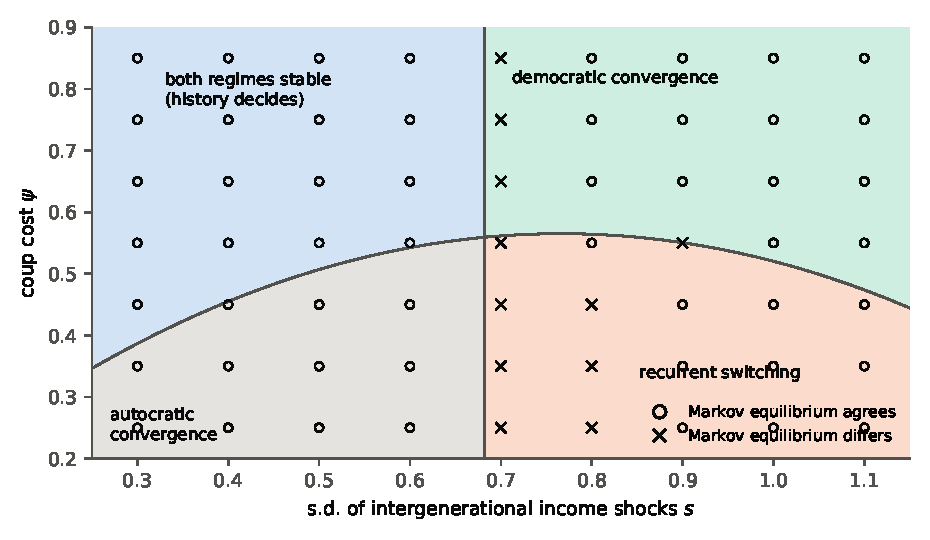
\includegraphics[width=0.85\textwidth]{figures/fig2_phase.pdf}
\caption{Phase diagram in (luck $s$, coup cost $\psi$) space, with $\mu=0.35$.  Regions use the closed-form boundaries $s=\bar s$ \eqref{eq:sbar} and $\psi=\psi_c(s)$.  Markers: long-run outcome of the numerical Markov equilibrium from both initial regimes ($p=q=0.3$, no concessions); circles agree with the closed form, crosses do not.}
\label{fig:phase}
\end{figure}

\begin{observation}[Cross-regime anticipation]\label{obs:anticipation}
On a $9\times7$ grid (Figure~\ref{fig:phase}), the Markov equilibrium agrees with the closed-form taxonomy at 52 of 63 points.  All 11 disagreements lie to the right of $\bar s$ ($s\in\{0.7,0.8,0.9\}$), and in every one the equilibrium is \emph{more stable} than the permanent-value conditions predict.  Three of the 11 come from converged solutions ($s=0.7$, $\psi\le0.45$).  There autocracy survives where the closed form predicts recurrent switching: the masses will not pay $\mu$ for a democracy that coups will overturn.  The other eight sit near a boundary where the iteration does not converge (Section~\ref{sec:numerics}), so they are suggestive only.  The converse channel shows up cleanly in the coup threshold.  With autocracy absorbing it is $0.621$ ($\psi=0.45$); when autocracy is itself exposed to revolution ($q=0.3$, $\mu=0.05$, no concessions) it rises to $0.675$, because the elite gains less from a coup into an autocracy that will later fall.  This interaction is invisible when either side is held fixed.
\end{observation}

\begin{figure}[t]
\centering
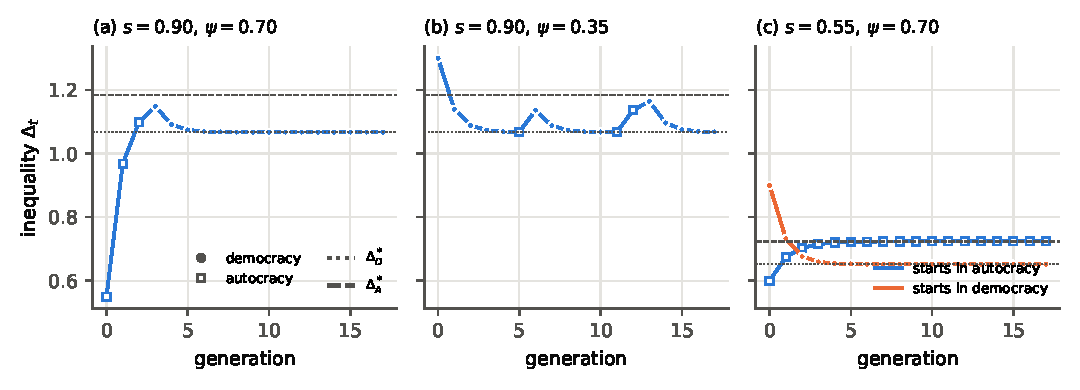
\includegraphics[width=\textwidth]{figures/fig3_paths.pdf}
\caption{Simulated paths of inequality; filled circles mark democracy, open squares autocracy.  (a) Democratic convergence ($s=0.90$, $\psi=0.70$): inequality builds up under autocracy until the revolution threat binds, then democracy compresses it.  (b) Recurrent switching ($s=0.90$, $\psi=0.35$): democracy cannot compress inequality out of the coup zone.  (c) History dependence ($s=0.55$, $\psi=0.70$): identical primitives, different initial regimes, different long-run regime and inequality.}
\label{fig:paths}
\end{figure}

\subsection{Numerical method and diagnostics}\label{sec:numerics}

Values $W(\Delta^2,r)$ and $B(\Delta^2,r)$ live on a 700-point grid in $\Delta^2\in[0.02,3.5]$, with linear interpolation.  Decision rules are best responses to current values, and values are updated by damped iteration (damping $0.5$).  Away from region boundaries the iteration converges (sup-norm change below $10^{-9}$).  The closed-form thresholds are reproduced whenever the destination regime is absorbing: $0.621$ for $\psi=0.45$ and $0.943$ for $\psi=0.62$.  Near boundaries, where a switching threshold coincides with a steady state, the rule toggles at a few grid points and the iteration does not converge.  This is the same symptom as in Observation~\ref{obs:productive} and suggests mixed strategies on a thin set.  Code and figures are in \texttt{code/}.

%=====================================================================
\section{What the core says to the one-sided literatures}\label{sec:empirics}
%=====================================================================

These are model implications, not established facts; each needs an empirical design.

\begin{enumerate}
\item \textbf{Democracy $\to$ inequality.}  Relative to the autocratic counterfactual, democratization always lowers inequality here ($\rho_\D<\rho_\A$).  But the \emph{before--after} change is
\[
\Delta^2_{t+k}-\Delta^2_0=(1-\rho_\D^{2k})(\Delta^{*2}_\D-\Delta^2_0),
\]
which is positive when an autocracy starts below the democratic steady state (e.g.\ after a leveling shock) and negative otherwise.  This is the ``convergence to the middle'' found by \citet{DorschMaarek2019}.  Averaged over heterogeneous starting points, it can produce the null average effect documented by \citet{AcemogluEtAl2015Handbook}.
\item \textbf{Inequality $\to$ regime.}  Breakdown risk is increasing in inequality on the distributive branch (the coup zone), consistent with \citet{Houle2009} and \citet{RauStokes2024}.  The democratization side is weaker in the model because of anticipation (Observation~\ref{obs:anticipation}) and inequality management (M2).  Both flatten the reduced-form relation, consistent with Houle's null for democratization.  This is a possibility result, not a derivation.
\item \textbf{Income/inequality and democracy with fixed effects.}  Long-run regimes are functions of country primitives ($s$, $\psi$, $\mu$, $z$, $\beta$), which country fixed effects absorb.  Within-country variation moves the regime only near thresholds.  This is one way to read \citet{AcemogluEtAl2008} alongside the strong cross-sectional correlation.  Compare the reconciliation in \citet{CervellatiEtAl2025}, which works through growth rather than distributional states.
\item \textbf{A sharp test.}  Corollary~\ref{cor:democap}(ii): conditional on current inequality (and primitives), democratic history should not predict breakdown.  Values-based persistence predicts the opposite.
\end{enumerate}

%=====================================================================
\section{Literature positioning}\label{sec:lit}
%=====================================================================

\begin{longtable}{p{0.24\textwidth}p{0.33\textwidth}p{0.33\textwidth}}
\toprule
Paper & What it does & Relation to the core\\
\midrule
\endhead
\citet{Benabou1996,Benabou2000,Benabou2002} & Log-normal dynamics, constant-elasticity redistribution, credit constraints; political bias $\lambda$; US/Europe multiple steady states & The workhorse.  As far as I can tell, $\lambda$ is a primitive and regimes do not change (to be verified against the text).\\
\citet{HasslerEtAl2003} & Redistribution shapes the future electorate; survival of the welfare state & Policy--electorate feedback within a fixed democracy.\\
\citet{AcemogluRobinson2000,AcemogluRobinson2001,AcemogluRobinson2006,AcemogluRobinson2008} & Democracy as commitment; coups; captured democracy; Kuznets narrative & Transition technology for the core; inequality is a parameter or evolves outside a distributional state.\\
\citet{JustmanGradstein1999} & Industrialization $\to$ franchise $\to$ redistribution $\to$ falling inequality in Britain & The historical loop the core formalizes.\\
\citet{JackLagunoff2006}; \citet{Leventoglu2014}; \citet{AcemogluEgorovSonin2018} & Franchise as delegation; mobility and transitions & M3, with exogenous mobility; here mobility is $\rho(\tau)$.\\
\citet{PerssonTabellini2009} & Democratic capital and exit hazards & Corollary~\ref{cor:democap} derives the stock.\\
\citet{BenhabibPrzeworski2006} & Democracy survives when redistribution can satisfy rich and poor & Income-level threshold; no distributional state.\\
\citet{BourguignonVerdier2000}; \citet{CervellatiEtAl2025}; \citet{BoucekkineEtAl2026Unified} & Education/growth and regimes & Aggregate human capital rather than a dispersion state.\\
\citet{Grossman1994}; \citet{Albertus2015}; \citet{Paglayan2021} & Land reform and mass education under autocracy & M2's inequality management.\\
\citet{DorschMaarek2019}; \citet{Houle2009}; \citet{RauStokes2024}; \citet{AcemogluEtAl2008,AcemogluEtAl2015Handbook,AcemogluEtAl2019JPE} & One-sided empirical facts & Section~\ref{sec:empirics}.\\
\bottomrule
\end{longtable}

\paragraph{Novelty, stated carefully.}  The loop from inequality to franchise to redistribution and back to inequality is old (Acemoglu--Robinson; Justman--Gradstein).  What I have not found is:
\begin{enumerate}[label=(\roman*)]
\item regime transitions embedded in B\'enabou's exact-aggregation dynamics, giving closed-form regime surpluses;
\item the decomposition of the elite's surplus into the median's surplus minus a dynastic stake;
\item the derivation of democratic capital as the inequality gap, with its depreciation rate pinned to intergenerational persistence.
\end{enumerate}
This is a search-based claim, and the search was narrower than the previous note's.

%=====================================================================
\section{Assumption ledger and next steps}
%=====================================================================

\begin{longtable}{p{0.3\textwidth}p{0.2\textwidth}p{0.4\textwidth}}
\toprule
Assumption & Role & Comment\\
\midrule
\endhead
Credit-constrained investment out of post-tax income ($\beta>0$) & mechanism-essential & Makes persistence policy-dependent; without it the distribution does not respond to the regime.\\
Regime determines who decides (de jure control) & mechanism-essential & Source of the commitment value of a regime.\\
Random opportunities $p,q<1$; costs $\psi,\mu$ & substantive & Make regimes sticky; with free, frequent reversal democracy is a one-period policy (Obs.~\ref{obs:productive}).\\
Fixed policy menu $(\tau_\A,\tau_\D)$ & substantive / tractability & Matters most for voluntary transitions; M5 relaxes it.\\
Rank-defined elite and median masses & substantive & Builds in mobility; a fixed-membership class would remove M3.\\
Log-normality, constant investment share, $d(\tau)$ quadratic & tractability & Exact aggregation; non-log utility needed for hold-up (M4).\\
Generation-length periods & tractability & Weakens Acemoglu--Robinson commitment problems; overlapping cohorts fix it.\\
\bottomrule
\end{longtable}

\paragraph{Recommended sequence.}
\begin{enumerate}
\item Write the core as a short theory paper: Propositions~\ref{prop:surplus}--\ref{prop:taxonomy}, the loop-sign table, and Corollary~\ref{cor:democap}.  Prove that the elite stages a coup at every opportunity inside the zone, using the regression of descendants' positions to bound the option value of waiting.
\item Add endogenous democratic policy under the coup constraint (M5).  This is where the most interesting new result probably lies: captured versus consolidated democracy, with redistribution rising in democratic age.
\item Replace generations with overlapping cohorts so that hazards are measured in years, and revisit concessions (M2) once the commitment problem has bite.
\item Empirical companion: test Corollary~\ref{cor:democap}(ii) and the conditional dynamics in Section~\ref{sec:empirics} on democratic spells.
\end{enumerate}

\paragraph{The three things to remember.}  (1) The regime/distribution loop runs through intergenerational persistence, which policy controls.  (2) A regime digs itself in when the inequality it creates weakens the group that can overturn it; democracy does so through the elite's shrinking dynastic stake.  (3) Democratic capital is the inequality gap, and its depreciation rate is the squared intergenerational elasticity.

%=====================================================================
\begin{thebibliography}{99}

\bibitem[Acemoglu et al.(2008)]{AcemogluEtAl2008}
Acemoglu, D., Johnson, S., Robinson, J.~A., and Yared, P. (2008).
Income and democracy.
\emph{American Economic Review}, 98(3), 808--842.

\bibitem[Acemoglu et al.(2015)]{AcemogluEtAl2015Handbook}
Acemoglu, D., Naidu, S., Restrepo, P., and Robinson, J.~A. (2015).
Democracy, redistribution, and inequality.
In A.~B. Atkinson and F.~Bourguignon (eds.), \emph{Handbook of Income Distribution}, Vol.~2B, 1885--1966.

\bibitem[Acemoglu et al.(2019)]{AcemogluEtAl2019JPE}
Acemoglu, D., Naidu, S., Restrepo, P., and Robinson, J.~A. (2019).
Democracy does cause growth.
\emph{Journal of Political Economy}, 127(1), 47--100.

\bibitem[Acemoglu et al.(2018)]{AcemogluEgorovSonin2018}
Acemoglu, D., Egorov, G., and Sonin, K. (2018).
Social mobility and stability of democracy: Reevaluating de Tocqueville.
\emph{Quarterly Journal of Economics}, 133(2), 1041--1105.

\bibitem[Acemoglu and Robinson(2000)]{AcemogluRobinson2000}
Acemoglu, D., and Robinson, J.~A. (2000).
Why did the West extend the franchise? Democracy, inequality, and growth in historical perspective.
\emph{Quarterly Journal of Economics}, 115(4), 1167--1199.

\bibitem[Acemoglu and Robinson(2001)]{AcemogluRobinson2001}
Acemoglu, D., and Robinson, J.~A. (2001).
A theory of political transitions.
\emph{American Economic Review}, 91(4), 938--963.

\bibitem[Acemoglu and Robinson(2006)]{AcemogluRobinson2006}
Acemoglu, D., and Robinson, J.~A. (2006).
\emph{Economic Origins of Dictatorship and Democracy}.
Cambridge University Press.

\bibitem[Acemoglu and Robinson(2008)]{AcemogluRobinson2008}
Acemoglu, D., and Robinson, J.~A. (2008).
Persistence of power, elites, and institutions.
\emph{American Economic Review}, 98(1), 267--293.

\bibitem[Albertus(2015)]{Albertus2015}
Albertus, M. (2015).
\emph{Autocracy and Redistribution: The Politics of Land Reform}.
Cambridge University Press.

\bibitem[Ansell and Samuels(2014)]{AnsellSamuels2014}
Ansell, B.~W., and Samuels, D.~J. (2014).
\emph{Inequality and Democratization: An Elite-Competition Approach}.
Cambridge University Press.

\bibitem[B\'enabou(1996)]{Benabou1996}
B\'enabou, R. (1996).
Heterogeneity, stratification, and growth: Macroeconomic implications of community structure and school finance.
\emph{American Economic Review}, 86(3), 584--609.

\bibitem[B\'enabou(2000)]{Benabou2000}
B\'enabou, R. (2000).
Unequal societies: Income distribution and the social contract.
\emph{American Economic Review}, 90(1), 96--129.

\bibitem[B\'enabou(2002)]{Benabou2002}
B\'enabou, R. (2002).
Tax and education policy in a heterogeneous-agent economy: What levels of redistribution maximize growth and efficiency?
\emph{Econometrica}, 70(2), 481--517.

\bibitem[Benhabib and Przeworski(2006)]{BenhabibPrzeworski2006}
Benhabib, J., and Przeworski, A. (2006).
The political economy of redistribution under democracy.
\emph{Economic Theory}, 29(2), 271--290.

\bibitem[Boix(2003)]{Boix2003}
Boix, C. (2003).
\emph{Democracy and Redistribution}.
Cambridge University Press.

\bibitem[Boucekkine et al.(2026)]{BoucekkineEtAl2026Unified}
Boucekkine, R., Desbordes, R., Ruan, W., and Zou, B. (2026).
A unified theory of institutional dynamics.
AMSE Working Paper 2026-13.

\bibitem[Bourguignon and Verdier(2000)]{BourguignonVerdier2000}
Bourguignon, F., and Verdier, T. (2000).
Oligarchy, democracy, inequality and growth.
\emph{Journal of Development Economics}, 62(2), 285--313.

\bibitem[Cervellati et al.(2025)]{CervellatiEtAl2025}
Cervellati, M., Meyerheim, G., and Sunde, U. (2025).
Income, democracy and growth: Reconciling evidence and theory.
\emph{Economic Journal}, article ueaf112.

\bibitem[Dorsch and Maarek(2019)]{DorschMaarek2019}
Dorsch, M.~T., and Maarek, P. (2019).
Democratization and the conditional dynamics of income distribution.
\emph{American Political Science Review}, 113(2), 385--404.

\bibitem[Galor and Zeira(1993)]{GalorZeira1993}
Galor, O., and Zeira, J. (1993).
Income distribution and macroeconomics.
\emph{Review of Economic Studies}, 60(1), 35--52.

\bibitem[Grossman(1994)]{Grossman1994}
Grossman, H.~I. (1994).
Production, appropriation, and land reform.
\emph{American Economic Review}, 84(3), 705--712.

\bibitem[Hassler et al.(2003)]{HasslerEtAl2003}
Hassler, J., Rodr\'iguez Mora, J.~V., Storesletten, K., and Zilibotti, F. (2003).
The survival of the welfare state.
\emph{American Economic Review}, 93(1), 87--112.

\bibitem[Heathcote et al.(2017)]{HeathcoteStoreslettenViolante2017}
Heathcote, J., Storesletten, K., and Violante, G.~L. (2017).
Optimal tax progressivity: An analytical framework.
\emph{Quarterly Journal of Economics}, 132(4), 1693--1754.

\bibitem[Houle(2009)]{Houle2009}
Houle, C. (2009).
Inequality and democracy: Why inequality harms consolidation but does not affect democratization.
\emph{World Politics}, 61(4), 589--622.

\bibitem[Jack and Lagunoff(2006)]{JackLagunoff2006}
Jack, W., and Lagunoff, R. (2006).
Dynamic enfranchisement.
\emph{Journal of Public Economics}, 90(4--5), 551--572.

\bibitem[Justman and Gradstein(1999)]{JustmanGradstein1999}
Justman, M., and Gradstein, M. (1999).
The industrial revolution, political transition, and the subsequent decline in inequality in 19th-century Britain.
\emph{Explorations in Economic History}, 36(2), 109--127.

\bibitem[Levento\u{g}lu(2014)]{Leventoglu2014}
Levento\u{g}lu, B. (2014).
Social mobility, middle class, and political transitions.
\emph{Journal of Conflict Resolution}, 58(5), 825--864.

\bibitem[Paglayan(2021)]{Paglayan2021}
Paglayan, A.~S. (2021).
The non-democratic roots of mass education: Evidence from 200 years.
\emph{American Political Science Review}, 115(1), 179--198.

\bibitem[Persson and Tabellini(2009)]{PerssonTabellini2009}
Persson, T., and Tabellini, G. (2009).
Democratic capital: The nexus of political and economic change.
\emph{American Economic Journal: Macroeconomics}, 1(2), 88--126.

\bibitem[Rau and Stokes(2024)]{RauStokes2024}
Rau, E.~G., and Stokes, S. (2024).
Income inequality and the erosion of democracy in the twenty-first century.
\emph{Proceedings of the National Academy of Sciences}, doi:10.1073/pnas.2422543121.

\end{thebibliography}

\end{document}
